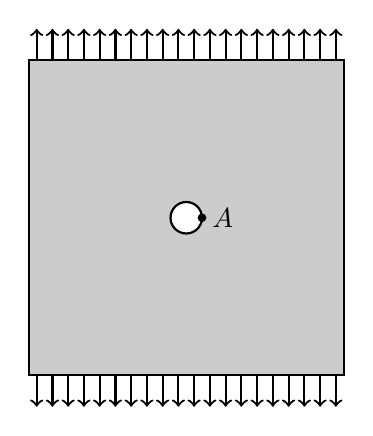
\begin{tikzpicture}[thick, scale = 0.4]
\draw [fill=gray!40!white] (0, 0) -- (10, 0) -- (10, 10) -- (0, 10) -- cycle;
\draw [fill=white] (5, 5) circle (0.5);
\foreach \x in {0,...,19}{
	\draw[->] (0.25+0.5*\x, 0) -- (0.25+0.5*\x, -1);
	\draw[->] (0.25+0.5*\x, 10) -- (0.25+0.5*\x, 11);}
	\draw[fill=black] (5.5, 5) circle (0.1) node [right] {$A$};

\end{tikzpicture}